%Notes by Harsh Mistry 
%Math 239
%based on Template from : https://www.cs.cmu.edu/~ggordon/10725-F12/template.tex

\documentclass{article}
\setlength{\oddsidemargin}{0.25 in}
\setlength{\evensidemargin}{-0.25 in}
\setlength{\topmargin}{-0.6 in}
\setlength{\textwidth}{6.5 in}
\setlength{\textheight}{8.5 in}
\setlength{\headsep}{0.75 in}
\setlength{\parindent}{0 in}
\setlength{\parskip}{0.1 in}
\usepackage{amsfonts,graphicx, amssymb}
\usepackage[fleqn]{amsmath}
\usepackage{fixltx2e}
\usepackage{color}
\graphicspath{ {images/} }
\usepackage{tcolorbox}
\usepackage{lipsum}
\usepackage{listings}
\usepackage{scrextend}
\tcbuselibrary{skins,breakable}
\usetikzlibrary{shadings,shadows}
\newcounter{lecnum}
\renewcommand{\thepage}{\thelecnum-\arabic{page}}
\renewcommand{\thesection}{\thelecnum.\arabic{section}}
\renewcommand{\theequation}{\thelecnum.\arabic{equation}}
\renewcommand{\thefigure}{\thelecnum.\arabic{figure}}
\renewcommand{\thetable}{\thelecnum.\arabic{table}}
\newcommand{\lecture}[4]{
   \pagestyle{myheadings}
   \thispagestyle{plain}
   \newpage
   \setcounter{lecnum}{#1}
   \setcounter{page}{1}
   
   
%Info Box 
   \begin{center}
   \framebox{
      \vbox{\vspace{2mm}
    \hbox to 6.28in { {\bf Math 239 - Introduction to Combinatorics
	\hfill Spring 2017} }
       \vspace{4mm}
       \hbox to 6.28in { {\Large \hfill Lecture #1: #2  \hfill} }
       \vspace{2mm}
       \hbox to 6.28in { {\it Lecturer: #3 \hfill Notes By: #4} }
      \vspace{2mm}}
   }
   \end{center}
   
   \markboth{Lecture #1: #2}{Lecture #1: #2}



 
}

\renewcommand{\cite}[1]{[#1]}
\def\beginrefs{\begin{list}%
        {[\arabic{equation}]}{\usecounter{equation}
         \setlength{\leftmargin}{2.0truecm}\setlength{\labelsep}{0.4truecm}%
         \setlength{\labelwidth}{1.6truecm}}}
\def\endrefs{\end{list}}
\def\bibentry#1{\item[\hbox{[#1]}]}

\newcommand{\fig}[3]{
			\vspace{#2}
			\begin{center}
			Figure \thelecnum.#1:~#3
			\end{center}
	}
	
	\newcommand{\bs}{
		\texttt{\char`\\ \hspace{0.1cm}} 
	}
	

	
\newcommand{\pipe}{\(\mid\)}
\newcommand{\ctr}{\(\wedge\)}

\newtheorem{theorem}{Theorem}[lecnum]
\newtheorem{lemma}[theorem]{Lemma}
\newtheorem{ex}[theorem]{Example}
\newtheorem{expx}[theorem]{Problem}
\newtheorem{prop}[theorem]{Proposition}
\newtheorem{claim}[theorem]{Claim}
\newtheorem{corollary}[theorem]{Corollary}
\newtheorem{definition}[theorem]{Definition}
\newenvironment{proof}{{\bf Proof:}}{\hfill\rule{2mm}{2mm}}
\newcommand\E{\mathbb{E}}

%color definitions :
\definecolor{darkred}{rgb}{0.55, 0.0, 0.0}
\definecolor{lightcoral}{rgb}{0.94, 0.5, 0.5}
\definecolor{tomato}{rgb}{1.0, 0.39, 0.28}
\definecolor{lightgray}{rgb}{.9,.9,.9}
\definecolor{darkgray}{rgb}{.4,.4,.4}
\definecolor{purple}{rgb}{0.65, 0.12, 0.82}
\definecolor{lightgreen}{rgb}{0.56, 0.93, 0.56}
\definecolor{darkgreen}{rgb}{0.0, 0.2, 0.13}
\definecolor{limegreen}{rgb}{0.2, 0.8, 0.2}
\definecolor{lightblue}{rgb}{0.68, 0.85, 0.9}
\definecolor{darkblue}{rgb}{0.0, 0.0, 0.55}


%Environments
\newenvironment{exblock}[1]{%
    \tcolorbox[beamer,%
    noparskip,breakable,
    colback=lightgreen,colframe=darkgreen,%
    colbacklower=limegreen!75!lightgreen,%
    title=#1]}%
    {\endtcolorbox}

\newenvironment{ablock}[1]{%
    \tcolorbox[beamer,%
    noparskip,breakable,
    colback=lightcoral,colframe=darkred,%
    colbacklower=tomato!75!lightcoral,%
    title=#1]}%
    {\endtcolorbox}

\newenvironment{cblock}[1]{%
    \tcolorbox[beamer,%
    noparskip,breakable,
    colback=lightblue,colframe=darkblue,%
    colbacklower=darkblue!75!lightblue,%
    title=#1]}%
    {\endtcolorbox}


%Languages
\lstdefinelanguage{JavaScript}{
  keywords={typeof, new, true, false, catch, function, return, null, catch, switch, var, if, in, while, do, else, case, break},
  keywordstyle=\color{blue}\bfseries,
  ndkeywords={class, export, boolean, throw, implements, import, this},
  ndkeywordstyle=\color{darkgray}\bfseries,
  identifierstyle=\color{black},
  sensitive=false,
  comment=[l]{//},
  morecomment=[s]{/*}{*/},
  commentstyle=\color{purple}\ttfamily,
  stringstyle=\color{red}\ttfamily,
  morestring=[b]',
  morestring=[b]"
}

%Listings
\lstset{
   language=JavaScript,
   backgroundcolor=\color{lightgray},
   extendedchars=true,
   basicstyle=\footnotesize\ttfamily,
   showstringspaces=false,
   showspaces=false,
   numbers=left,
   numberstyle=\footnotesize,
   numbersep=9pt,
   tabsize=2,
   breaklines=true,
   showtabs=false,
   captionpos=b
}


%Start
\begin{document}

\lecture{16}{June 5th, 2017}{Alan Arroyo Guevara}{Harsh Mistry}

\section{Graph Theory}
\begin{definition}
A graph G is a pair G=(V,E), where B is an finite set, called the vertices of G, and E is a set of unordered pairs (2-sets) of elements in V, called the edges of G. 
\end{definition}

\begin{ex}
\[V = \langle a, b, c, d, e\rangle\]
\[E = \langle \{a,b\}, \{b,c\}, \{c,d\}, \{d, a\}, \{a, e\}\rangle\]
\begin{center}
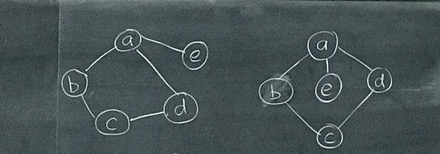
\includegraphics[scale=0.5]{1}
\end{center}
\end{ex}

In drawings of graphs, vertices are represented as points in the plan an edges are arcs connecting them.

\begin{ablock}{Remarks}
\begin{itemize}
\item Instead of saying "edge \(\{u,v\}\)", we say "edge uv"
\item Also \(V(G) = V\) and \(E(G) = E\)
\item We also don't study graphs with multiple edges or loops 
\end{itemize}
\end{ablock}

\subsection*{Terminology}
Let G be a graph an \(e = uv \in E(G)\), we say 
\begin{itemize}
\item u and v are \underline{adjacent}
\item v is a \underline{neighbour} of u
\item e is \underline{incident} to u
\item e is \underline{joins} u and v
\end{itemize}

\begin{ex}-\\
\begin{itemize}
\item a and b are adjacent 
\item a and d are not adjacent 
\item j has no neighbours 
\item bf  is incident with f.
\end{itemize}
\begin{center}
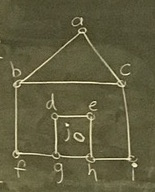
\includegraphics[scale=0.5]{2}
\end{center}
\end{ex}

Graphs can also be used to represent interesting objects 

\begin{ex}(Cubes) \\
Let k be a positive integer and define \(Q_k = (V,E)\)
\[V = \{0,1\} strings of length k\]
\[E = S_1 S_2 : S_1 S_2 \in V, s_1 \text{ and } s_2 \text{ differ in at most one digit}\]
\begin{center}
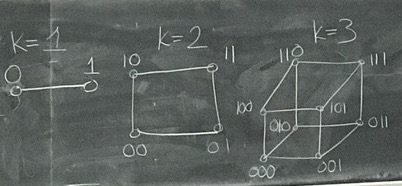
\includegraphics[scale=0.5]{3}
\end{center}
\end{ex}

\begin{ex} (Maps)
\textbf{Four Colour Conjecture} : Every map can be coloured using 4-colours, such that no two regions share a "real boundary" having the same colour.

\begin{center}
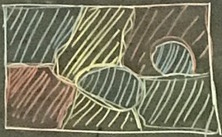
\includegraphics[scale=0.5]{4}
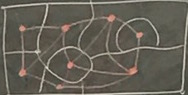
\includegraphics[scale=0.7]{5}
\end{center}
\newpage
\textbf{A Plane graph} is a graph drawn with no crossing between the edges. 
From every map you can get a plane graph 
\end{ex}

\subsection{Isomorphisms}
Are the following graphs the same : \\
\begin{center}
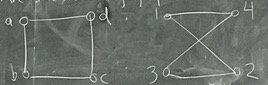
\includegraphics[scale=0.8]{6}
\end{center}
\begin{definition}
Two graphs \(G_1\) and \(G_2\) are isomorphic iff there exists a bijection 
$$ f : V(G_1) \longrightarrow V(G_2)$$
such that 
$$ uv \in E(G_1) \iff f(u)(v) \in E(G_2) $$
\end{definition}

\end{document}